\subsection{Use-case hệ thống}
    \begin{figure}[h]
        \centering
        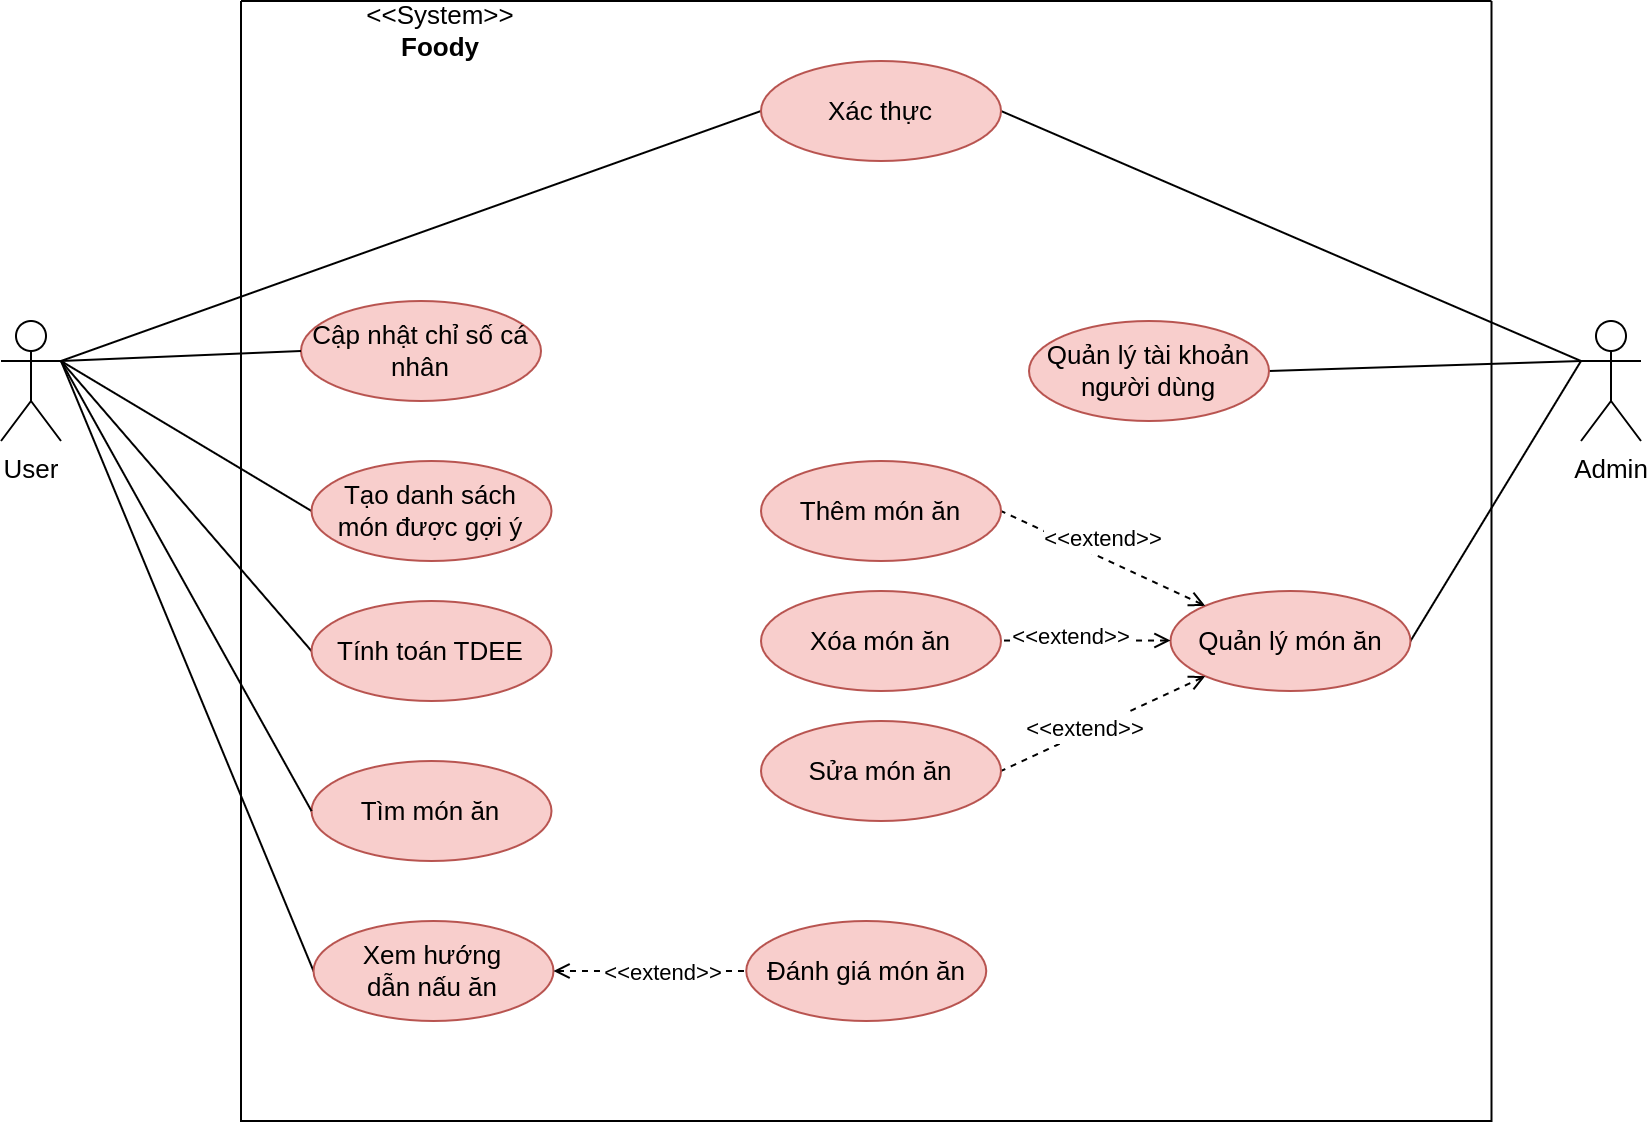
\includegraphics[width=1\linewidth]{images/use-case diagram/system_use-case.png}
        \caption{Use-case hệ thống}
    \end{figure}
    
    \begin{tblr}{
        width=1\linewidth,
        hlines,
        vlines,
        colspec={X[3]X[7]},
        columns = {valign = m, },
        row{1} = {halign = c, valign = m, bg = lightgray, fg = black},
    }
        {\textbf{Use case name} & \textbf{Tính toán TDEE}}  \\
        Description	 & 	Người dùng nhập các thông tin cần thiết để hệ thống tính toán TDEE và gợi ý mục tiêu cho người dùng \\
        Actor & Người dùng (User) \\
        Trigger & 	Người dùng ấn vào nút “Tính TDEE”\\
        Pre-condition & Người dùng đang ở trang chủ\\
        Post-condition & Hệ thống đưa ra chỉ số TDEE và mục tiêu của người dùng\\
        Normal flow &   1. Người dùng chuyển sang mục tính toán TDEE \newline
                    	2. Hệ thống hiển thị giao diện nhập thông tin \newline
                    	3. Người dùng nhập các thông tin cần thiết như tuổi, chiều cao, cân nặng, giới tính, mục tiêu \newline
                    	4. Người dùng ấn xác nhận \newline
                    	5. Hệ thống thực hiện tính toán và trả về kết quả \newline
                    	6. Hệ thống lưu thông tin vừa tính được vào cơ sở dự liệu \\
        Alternative flow  & None \\
        Exception flow & 	Exception flow thứ 1: Tại bước 3 \newline
                            1a Nếu người dùng nhập thông tin sai định dạng (ví dụ như tuổi là -3) hoặc chưa nhập thì bước 6 là: Hệ thống sẽ báo lỗi và yêu cầu người dùng nhập lại \\
    \end{tblr}
    
    \begin{tblr}{
        width=1\linewidth,
        hlines,
        vlines,
        colspec={X[3]X[7]},
        columns = {valign = m, },
        row{1} = {halign = c, valign = m, bg = lightgray, fg = black},
    }
        {\textbf{Use case name} & \textbf{Hướng dẫn người dùng từng bước nấu ăn}}  \\
        Description	 & 	Người dùng nhập các thông tin cần thiết để hệ thống tính toán TDEE và gợi ý mục tiêu cho người dùng \\
        Actor & Người dùng (User) \\
        Trigger & Người dùng nhấn vào nút “Hướng dẫn nấu ăn" \\
        Pre-condition & Người dùng đang ở trang lịch ăn trong ngày \\
        Post-condition & Hệ thống đưa ra hướng dẫn về nguyên liệu và cách nấu \\
        Normal flow &   1. Người dùng ấn vào “Lịch ăn” \newline
                    	2. Hệ thống lấy dữ liệu lịch ăn và hiển thị lên cho người dùng \newline
                    	3. Người dùng chọn một món ăn đã được lên lịch và ấn vào nút “Hướng dẫn nấu” \newline 
                    	4. Hệ thống lấy công thức từ Database rồi hiển thị lên cho người dùng.” \\
        Alternative flow  & None \\
        Exception flow & 	Exception flow thứ 1: Tại bước 4 \newline
                            1a. Nếu hệ thống tìm kiếm trong Database không có, thì sẽ hiển thị thông báo “Hiện chưa có hướng dẫn” cho người dùng \\
       Extended points & Đánh giá món ăn
    \end{tblr}
    
    \vspace{1cm}
    
    \begin{tblr}{
        width=1\linewidth,
        hlines,
        vlines,
        colspec={X[3]X[7]},
        columns = {valign = m, },
        row{1} = {halign = c, valign = m, bg = lightgray, fg = black},
    }
        {\textbf{Use case name} & \textbf{Đánh giá món ăn}}  \\
        Description	 & 	Người dùng đánh giá món ăn sau khi xem hướng dẫn nấu ăn \\
        Actor & Người dùng (User) \\
        Trigger & Người dùng xem hướng dẫn nấu món ăn và kéo xuống dưới cùng \\
        Pre-condition & Người dùng đang xem một hướng dẫn nấu ăn\\
        Post-condition & Hệ thống cập nhập đánh giá của người dùng vào database và cập nhập đánh giá tổng thể của món ăn\\
        Normal flow &   1. Ở hướng dẫn nấu ăn, người dùng kéo xuống bên dưới sẽ thấy phần đánh giá, sau                             đó người dùng chọn số sao muốn đánh giá và nhập bình luận của mình \newline
                    	2.Hệ thống hiện ra thông báo xác nhận đánh giá \newline
                    	3. Người dùng chọn “Đồng ý” \newline 
                    	4. Hệ thống cập nhập đánh giá của người dùng vào database và cập nhập đánh giá của người dùng vào đánh giá tổng của món ăn \\
        Alternative flow  & Alternative flow thứ 1: Tại bước 3 \newline
                            1a. Người dùng chọn “Hủy bỏ” thì bước 4 là: Hệ thống đóng thông báo và trở về trang đánh giá ở hướng dẫn nấu ăn \\
        Exception flow & None \\
    \end{tblr}
    
    \begin{tblr}{
        width=1\linewidth,
        hlines,
        vlines,
        colspec={X[3]X[7]},
        columns = {valign = m, },
        row{1} = {halign = c, valign = m, bg = lightgray, fg = black},
    }
        {\textbf{Use case name} & \textbf{Cập nhật chỉ số cá nhân}}  \\
        Description	 & 	Người dùng cập nhập thông tin định kỳ \\
        Actor & Người dùng (User) \\
        Trigger & Người dùng nhấn thông tin cá nhân \\
        Pre-condition & Người dùng đã từng nhập thông tin tính TDEE\\
        Post-condition & Hệ thống trả về chỉ số TDEE và gợi ý cho người dùng, sau đó cập nhập mới thông tin vào Database\\
        Normal flow &   1. Hệ thống hiển thị dấu chấm than màu vàng ở nút “Tính TDEE” \newline
                        2. Người dùng nhấn vào "Tính TDEE" \newline
                        3. Hệ thống chuyển hướng đến trang tính TDEE \newline
                        4. Người dùng nhập thông tin và nhấn vào nút "Tính TDEE" \newline
                    	5. Hệ thống thực hiện tính toán và trả về kết quả bao gồm chỉ số TDEE và mục tiêu gợi ý cho người dùng, sau đó cập nhập mới thông tin của người dùng vào Database và xóa dấu chấm than\\
        Alternative flow  & None \\
        Exception flow & None \\
    \end{tblr}
    
    \vspace{0.5cm}
    
    \begin{tblr}{
        width=1\linewidth,
        hlines,
        vlines,
        colspec={X[3]X[7]},
        columns = {valign = m, },
        row{1} = {halign = c, valign = m, bg = lightgray, fg = black},
    }
        {\textbf{Use case name} & \textbf{Tìm món ăn}}  \\
        Description	 & 	Người dùng tìm kiếm các món ăn trong hệ thống \\
        Actor & Người dùng (User) \\
        Trigger & Người dùng nhấn vào nút tìm kiếm \\
        Pre-condition & Người dùng đã đăng nhập \\
        Post-condition & Hệ thống trả về các món ăn theo từ khóa tìm kiếm \\
        Normal flow &   1. Hệ thống hiển thị giao diện tìm kiếm \newline
                        2. Người dùng nhập từ khóa món ăn \newline
                        3. Hệ thống tìm các món ăn có chứa từ khóa \newline
                        4. Hệ thống trả về dữ liệu tìm được \newline
                    	5. Hệ thống hiển thị danh sách các món ăn lên màn hình\\
        Alternative flow  & None \\
        Exception flow & Exception flow thứ 1: tại bước 3 \newline
                         1a. Nếu không tìm thấy món ăn, hệ thống thông báo cho người dùng\\
    \end{tblr}

    \vspace{0.5cm}
    
    \begin{tblr}{
        width=1\linewidth,
        hlines,
        vlines,
        colspec={X[3]X[7]},
        columns = {valign = m, },
        row{1} = {halign = c, valign = m, bg = lightgray, fg = black},
    }
        {\textbf{Use case name} & \textbf{Quản lý tài khoản người dùng}}  \\
        Description	 & 	Admin quản lý tài khoản đang có trong hệ thống \\
        Actor & Quản lý (Admin) \\
        Trigger & Quản lý ấn vào mục quản lý tài khoản \\
        Pre-condition & Quản lý đã đăng nhập \\
        Post-condition & Các tài khoản được quản lý \\
        Normal flow &   1. Hệ thống lấy thông tin về các tài khoản có trong hệ thống \newline
                        2. Hệ thống hiện danh sách các tài khoản \newline
                        3. Quản lý chọn tài khoản muốn quản lý \newline
                        4. Hệ thống hiển thị thông tin chi tiết của tài khoản \newline
                    	5. Quản lý chọn hành động (sửa, cấm) \newline 
                    	6. Hệ thống hiện thị thông báo xác nhận \newline 
                    	7. Hệ thống ghi nhận hành động của quản lý \\
        Alternative flow  & Alternative flow thứ 1: tại bước 6 \newline
                            1a. Nếu người dùng ấn hủy, quay lại bước 4\\
        Exception flow & none\\
    \end{tblr}
    
    \begin{tblr}{
        width=1\linewidth,
        hlines,
        vlines,
        colspec={X[3]X[7]},
        columns = {valign = m, },
        row{1} = {halign = c, valign = m, bg = lightgray, fg = black},
    }
        {\textbf{Use case name} & \textbf{Quản lý món ăn}}  \\
        Description	 & 	Admin quản lý các món ăn đang có trong hệ thống \\
        Actor & Quản lý (Admin) \\
        Trigger & Quản lý ấn vào mục quản lý món ăn \\
        Pre-condition & Quản lý đã đăng nhập \\
        Post-condition & Món ăn được quản lý \\
        Normal flow &   1. Hệ thống lấy thông tin về các món ăn \newline
                        2. Hệ thống hiện danh sách các món ăn \\
        Extended point & Thêm món ăn, Xóa món ăn, Sửa món ăn
    \end{tblr}
    
    \vspace{0.5cm}
    
    \begin{tblr}{
        width=1\linewidth,
        hlines,
        vlines,
        colspec={X[3]X[7]},
        columns = {valign = m, },
        row{1} = {halign = c, valign = m, bg = lightgray, fg = black},
    }
        {\textbf{Use case name} & \textbf{Thêm món ăn}}  \\
        Description	 & 	Admin thêm món ăn mới \\
        Actor & Quản lý (Admin) \\
        Trigger & Quản lý ấn vào thêm món ăn \\
        Pre-condition & Quản lý đang ở phần quản lý món ăn \\
        Post-condition & Món ăn mới được thêm vào \\
        Normal flow &   1. Hệ thống hiển thị giao diện nhập món ăn mới \newline
                        2. Người dùng nhập thông tin về món ăn \newline
                        3. Người dùng ấn tạo món ăn \newline
                        4. Hệ thống kiểm tra thông tin được nhập \newline
                        5. Hệ thống ghi nhận món ăn vào database \\
        Alternative flow & none\\
        Exception flow & Exception flow thứ 1: tại bước 4
                         1a. Nếu thông tin nhập không đúng, thông báo cho người dùng \newline 
                         Quay lại bước 2 \\
    \end{tblr}
    
    \vspace{0.5cm}
    
    \begin{tblr}{
        width=1\linewidth,
        hlines,
        vlines,
        colspec={X[3]X[7]},
        columns = {valign = m, },
        row{1} = {halign = c, valign = m, bg = lightgray, fg = black},
    }
        {\textbf{Use case name} & \textbf{Xóa món ăn}}  \\
        Description	 & 	Admin xóa món ăn trong hệ thống \\
        Actor & Quản lý (Admin) \\
        Trigger & Quản lý ấn vào xóa món ăn trong phần chi tiết món ăn \\
        Pre-condition & Quản lý đang ở phần quản lý món ăn \\
        Post-condition & Món ăn được xóa \\
        Normal flow &   1. Quản lý chọn món ăn muốn xóa \newline
                        2. Hệ thống hiển thị thông tin chi tiết món ăn \newline
                        3. Quản lý chọn nút xóa món ăn \newline
                        4. Hệ thống hiển thị thông báo xác nhận \newline
                        6. Người dùng chọn đồng ý \newline
                        5. Hệ thống ghi nhận xóa món ăn khỏi database \\
        Alternative flow &  Alternative flow thứ 1: tại bước 1 \newline
                            1a. Quản lý ấn vào nút 3 chấm \newline
                            1b. Hệ thống hiển thị các tùy chọn \newline
                            1c. Người dùng chọn xóa món ăn \newline
                            Tiếp tục bước 4 \newline
                            \newline
                            Alternative flow thứ 2: tại bước 5 \newline
                            2a. Nêu người dùng chọn hủy, quay lại trang thông tin chi tiết \\
        Exception flow & none\\
    \end{tblr}
    
    \begin{tblr}{
        width=1\linewidth,
        hlines,
        vlines,
        colspec={X[3]X[7]},
        columns = {valign = m, },
        row{1} = {halign = c, valign = m, bg = lightgray, fg = black},
    }
        {\textbf{Use case name} & \textbf{Sửa món ăn}}  \\
        Description	 & 	Admin chỉnh sửa món ăn trong hệ thống \\
        Actor & Quản lý (Admin) \\
        Trigger & Quản lý ấn vào chính sửa món ăn trong phần chi tiết món ăn \\
        Pre-condition & Quản lý đang ở phần quản lý món ăn \\
        Post-condition & Món ăn được chỉnh sửa \\
        Normal flow &   1. Quản lý chọn món ăn muốn chỉnh sửa \newline
                        2. Hệ thống hiển thị thông tin chi tiết món ăn \newline
                        3. Quản lý chọn nút chỉnh sửa món ăn \newline
                        4. Hệ thống hiển thị giao diện chỉnh sửa món ăn \newline
                        5. Người dùng nhập thông tin muốn chỉnh sửa \newline
                        6. Người dùng ấn cập nhật \newline
                        7. Hệ thống kiểm tra thông tin được nhập \newline
                        8. Hệ thống ghi nhận chỉnh sửa món ăn vào database \\
        Alternative flow &  Alternative flow thứ 1: tại bước 1 \newline
                            1a. Quản lý ấn vào nút 3 chấm \newline
                            1b. Hệ thống hiển thị các tùy chọn \newline
                            1c. Người dùng chọn chỉnh món ăn \newline
                            Tiếp tục bước 4 \newline
                            \newline
                            Alternative flow thứ 2: tại bước 5 \newline
                            2a. Nêu người dùng chọn hủy, quay lại trang thông tin chi tiết \\
        Exception flow & Exception flow thứ 1: tại bước 7 \newline
                         1a. Nếu thông tin nhập sai, thông báo cho người dùng \newline 
                         Quay lại bước 5\\
    \end{tblr}
\newpage